In this chapter, we analize the behaviors of the current task-affinity
implementation considering different architectures and benchmarks.  This
analysis is two fold: on one side it allows to understand why the current
task-affinity implementation is not effective on some architectures, e.g. the
Intel Xeon, on the other which are the points of task-affinity logic that can be
optimized in order to improve an application \emph{throughput and
predictability}.

%%%%%%%%%%%%%%%%%%%%%%%%%%%%%%%%%%%%%%%%%%%%%%%%%%%%%%%%%%%%%%%%%%%%%%%%%%%%%
\section{Scheduler architecture on 2.6.34}

Now I will briefly introduce which are the parts of the scheduling procedure 
interested by the task-affinity logic and which are the most important changes 
carried out from 2.6.31 kernel version to 2.6.34.

%-----------------------------------------------------------------------------
\subsection{Task wake up management}

The scheduling procedure for a task starts when it wakes up. A task can wake up
for different reasons, i.e. a semaphore becomes unlocked or a new task creation.  In all those cases different
kernel functions are called, but at the end they call the \texttt{try\_to\_wake\_up} function:

\lstset{basicstyle=\footnotesize, language=c, captionpos=b, frame=single, label=lis:APIttwu}
\lstinputlisting{API_ttwu.c}

where $p$ is the to be waken task.
This function follows these steps:

\begin{enumerate}
\item Disables kernel preemption, locks the runqueue where $p$ was last executed and check 
if $p$ is not already waken up and it is not already on a runqueue. In the first case the 
function releases lock and exits, in the second case the function check if a
\textit{push} is necessary. Further details about these if statements will be
describe thereafter. If the two checks fail, $p$'s state is changed in the TASK\_WAKING, the
lock on runqueue is released and \texttt{select\_task\_rq}, a wrapper for a 
class-specific \texttt{select\_task\_rq\_rt}, is called. The function 
\texttt{task\_waking} at line 2420 is class-specific and regards only Fair tasks.

\begin{figure}[h]
  \lstset{basicstyle=\footnotesize, language=c, captionpos=b, frame=single,label=lis:steps}
  \lstinputlisting{ttwu_steps.c}
  \label{code:steps_ttwu}
  \caption{A portion of the \texttt{try\_to\_wake\_up} method}
\end{figure}

\item \texttt{select\_task\_rq\_rt} choose on which cpu $p$ will be executed. It
calls \texttt{find\_lowest\_rq} that returns the best cpu where to put $p$. Criteria
used to choose the best cpu for $p$ will be described soon. When \texttt{select\_task\_rq\_rt} 
returns, check for cpuaffinity \footnote{On Linux it is possible decide on which
cpu a task can be executed. The set of cpus that can execute a task is called 
cpuaffinity of that task. Each task owns a mask called \textit{cpus\_allowed} 
that include all cpus where it can be executed, that is its cpuaffinity} and 
if selected cpu is online, in that case returns, otherwise calls 
\texttt{select\_fallback\_rq} that returns an any online cpu that "respects" 
$p$'s cpuaffinity.

\begin{figure}[h]
  \lstset{basicstyle=\footnotesize, language=c, captionpos=b, frame=single,label=lis:steps}
  \lstinputlisting{select_task.c}
  \label{code:select_task}
  \caption{A portion of the \texttt{select\_task\_rq} method}
\end{figure}

\item acquires the lock on selected runqueue, updates some $p$'s statistics, enqueues 
$p$ on selected runqueue and calls \texttt{check\_preempt\_rq\_rt} 

\begin{figure}[h]
  \lstset{basicstyle=\footnotesize, language=c, captionpos=b, frame=single,label=lis:steps}
  \lstinputlisting{ttwu_check.c}
  \label{code:check_preempt}
  \caption{A portion of the \texttt{try\_to\_wake\_up} method}
\end{figure}

\item checks if $p$ has priority greater than priority of the task currently
executed on the selected runqueue, in that case it calls the \texttt{need\_resched}
function in order to perform the context-switch on the selected runqueue at the
end of \texttt{try\_to\_wake\_up}.

\begin{figure}[h]
  \lstset{basicstyle=\footnotesize, language=c, captionpos=b, frame=single,label=lis:steps}
  \lstinputlisting{check_prio.c}
  \label{code:prio_ttwu}
  \caption{A portion of the \texttt{check\_preempt\_curr} method}
\end{figure}

\item updates $p$'s state to TASK\_RUNNING and calls the class-specific function 
\texttt{task\_woken} to check if $p$ must be pushed from the selected runqueue.
\texttt{task\_woken} has effects only for Real-time tasks.

\begin{figure}[h]
  \lstset{basicstyle=\footnotesize, language=c, captionpos=b, frame=single,label=lis:steps}
  \lstinputlisting{final_ttwu.c}
  \label{code:final_ttwu}
  \caption{A portion of the \texttt{try\_to\_wake\_up} method}
\end{figure}

\end{enumerate}

The most important differences from version 2.6.31 related to Real-time tasks regard principally \texttt{try\_to\_wake\_up}.

It is possible to have multiple istances of \texttt{try\_to\_wake\_up} for the same task executed simultaneously. In the 2.6.31 kernel version, 
this problem is resolved by holding the runqueue lock. In the 2.6.34 kernel version, to deal with this issue a new task's state named TASK\_WAKING 
was introduced.

\begin{figure}[h]
  \lstset{basicstyle=\footnotesize, language=c, captionpos=b, frame=single,label=lis:steps}
  \lstinputlisting{state_list.c}
  \label{code:task_states}
  \caption{Task's states}
\end{figure}

TASK\_WAKING is used to indicate someone is already waking up the task, in this way other instances of \texttt{try\_to\_wake\_up} fail when executing 
the if statement at line 2396 of the \texttt{try\_to\_wake\_up}, Fig. \ref{code:steps_ttwu}, because the input parameter $state$ of 
\texttt{try\_to\_wake\_up} is in the most cases equal to TASK\_ALL and then, according to Fig. \ref{code:task_states}, 
\texttt{TASK\_WAKING \& TASK\_ALL} returns 0 and \texttt{try\_to\_wake\_up} exits. With this solution it is possible to reduce the time in which the 
lock of runqueue is held. 

%-----------------------------------------------------------------------------
\subsection{Migration policy}

Another important part of scheduling procedure is the migration policy. Migration of Real-time tasks is made in two ways: 

\begin{description}
\item[Push tasks:] The push operation is implemented by \texttt{push\_rt\_task()}. The function receives in input a runqueue and looks at the 
highest-priority non-running runnable real-time task on the input runqueue and considers all the runqueues to find a cpu where it can run. It 
searches for a runqueue that is of lower priority, that is, one where the currently running task can be preempted by the task that is being pushed. 

The research and the choice of the best cpu for the task to push is executed by \texttt{find\_lowest\_rq} the same function used in 
\texttt{select\_task\_rq\_rt}. This function builds a mask of cpus that contains the lowest-priority runqueues and returns the cpu on which the task 
to push has last executed, as it is likely to be cache-hot in that location. If this is not possible, the \texttt{sched\_domain} map is considered 
to find a CPU that is logically closest to last cpu that has executed the task to push. If this fails too, a cpu is selected randomly from the mask.

The push operation is performed until a real-time task fails to be migrated or there are no more tasks to be pushed. Because the algorithm always 
selects the highest non-running task for pushing, the assumption is that, if it cannot migrate it, then most likely the lower real-time tasks cannot 
be migrated either and the search is aborted. No lock is taken when scanning for the lowest-priority runqueue. When the target runqueue is found, 
only the lock of that runqueue is taken, after which a check is made to verify whether it is still a candidate to which to push the task (as the 
target runqueue might have been modified by a parallel scheduling operation on another CPU). If not, the search is repeated for a maximum of three 
trials, after which it is aborted. 

In order to decide which tasks must be pushed, a linked list named \textit{pushable\_list} is added to each runqueue. \texttt{push\_rt\_task()} 
selects tasks to push from this list. A task is inserted in this list when it is enqueued on a runqueue as show in the snippet below.

\begin{figure}[h]
  \lstset{basicstyle=\footnotesize, language=c, captionpos=b, frame=single, label=lis:steps}
  \lstinputlisting{enqueue_push.c}
  \label{code:ttwu}
  \caption{A portion of the \texttt{enqueue\_task\_rt} method}
\end{figure}

The current task of any runqueue can't never be in a pushable list, in fact, during a context switch the next task to be executed is removed from the 
runqueue's pushable list.

\item[Pull task:] The pull operation is implemented by \texttt{pull\_rt\_task()}. The algorithm looks at all the overloaded runqueues in the system 
and checks whether they have a Real-time task that can run on the current runqueue (that is, checks if the target cpu "respects" the cpuaffinity of 
the task to pull) and if that Real-time task is of a priority higher than the task the target runqueue is about to schedule. If so, the task is 
queued on the current runqueue. This search aborts only after scanning all the overloaded runqueues in the system. 

\end{description}

In the 2.6.34 kernel version, the migration logic and all data structures involved are not changed with respect to 2.6.31 version.

%%%%%%%%%%%%%%%%%%%%%%%%%%%%%%%%%%%%%%%%%%%%%%%%%%%%%%%%%%%%%%%%%%%%%%%%%%%%%
\section{Test computers and benchmarks}

In this section I will briefly describe machines and the benchmark used to test task-affinity.

\begin{figure}[htbp]
 \centering%
 \subfigure[Machine A: Intel Xeon E5440 \label{fig:Xeon}]%
  {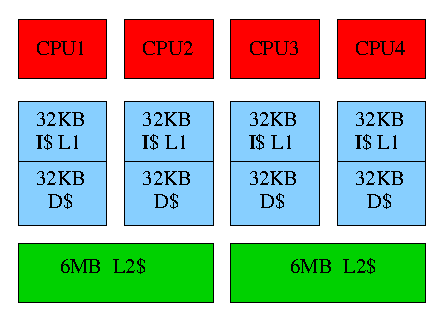
\includegraphics[width=6cm,height=8cm, keepaspectratio]{images/Xeon.eps}} \qquad\qquad
 \subfigure[Machine B: Intel i7 870 \label{fig:i7}]%
  {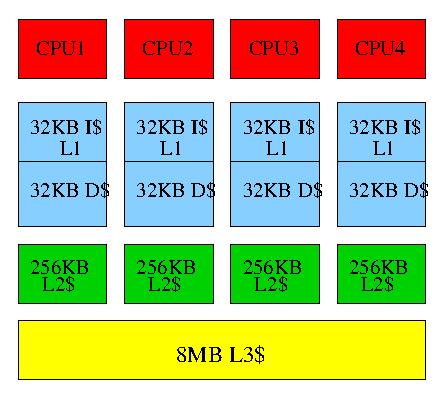
\includegraphics[width=6cm,height=8cm, keepaspectratio]{images/i7.eps}}
 \caption{\figurecaption{Cache configurations on computers used in this work. Those with D\$ are data cache, those with I\$ are instruction caches and 
the others are unified, that is, cache serves to data and instructions.
 }}
\end{figure}

\begin{description}
\item[Machine A] The first machine is an Intel Xeon E5440 running at 2.83GHz. There is not any cache shared among all cores. The LLC consists in two 
big L2-caches, of 6MB each, shared between sets of 2 cores cache hierarchy is shown in Fig. \ref{fig:Xeon}. On this machine there are two dies: CPU0 and 
CPU1 are on the same die, while other CPUs are on other die.

\item[Machine B] The second machine is an Intel Core i7 870 processor. It runs at 2.93 GHz and has the cache configuration as illustrated in Fig. 
\ref{fig:i7}. The LLC consists in one L3 of 8MB, which is shared by all cores. The L2-caches are private to each processor. All CPUs are on the same die.

\end{description}

The Benchmark used is the same as used in master thesis \cite{lcs}, in Fig.\ref{fig:bench} is represented its structure.

\begin{figure}[htbp]
\centering
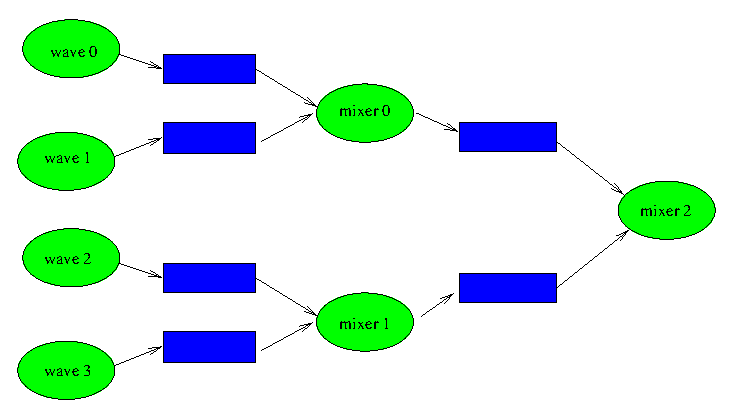
\includegraphics[width=\widefigure]{images/bench.eps}
\caption{\figurecaption{Structure of benchmark used: task are green coloured, buffer are blue coloured}}
\label{fig:bench}
\end{figure}

The Execution of benchmark is divided in three steps:

\begin{enumerate}
\item Waves write their buffer
\item Mixers read data from two buffers filled by waves, they mix read data and write them on their buffer, for example \textit{mixer0} reads data 
from the buffer filled by \textit{wave0} and from the buffer filled by wave1, mixes the data and then writes its buffer.
\item The Last mixer, reads data from the buffers written by \textit{mixer0} and \textit{mixer1}, mixes the data and writes its buffer.
\end{enumerate}

When \textit{mixer2} has finished to write data on its buffer, we say that a \textit{sample} was produced. The execution time to produce a sample 
depends on the buffers dimension, because each task has to fill its buffer. Note that waves fill their buffers with integers of 2 byte, therefore if 
buffer is of 4KB they will write 2048 integers in their buffer. Buffer dimension is always a power of 2.
The metric used to evaluate benchmark performance is the same as used in \cite{lcs}: 
\begin{equation}
	average + 2*standard deviation (A2S), 
\label{eq:metric_rt}
\end{equation}

where \textit{average} is the average of execution time to produce a sample and \textit{standard deviation} is the standard deviation of execution 
time to produce a sample. With this metric is possible measure throughput and predictability of the application.

%%%%%%%%%%%%%%%%%%%%%%%%%%%%%%%%%%%%%%%%%%%%%%%%%%%%%%%%%%%%%%%%%%%%%%%%%%%%%
\section{Analysis of Taskaffinity behaviour}

This section analyzes which are the improvements and downsides that the current version of task-affinity shows on different test computers and various
buffer dimensions.

In the following experiments only the Intel Xeon and Intel i7 architectures are considered, because their cache architectures are similar in structure.
These architectures differing in inter-chip communication, the former uses Quick-path Interconnect (QPI) the latter uses Hyper-transport (HT). 
Furthermore, Intel i7 uses an inclusive LLC with MESIF protocol. To observe how these factors impact on task-affinity a complex analysis would be required 
and this is not the goal of this thesis.
 
%-----------------------------------------------------------------------------
\subsection{Application's performance}

The length of the buffers determine how long the work executed by producers and consumers takes. It was showed in \cite{lcs} that if buffers used are 
too short and consequently tasks have very few work to do in user-space side, the parallelism provided by the SMP system is not well profited. For 
this reason, in \cite{lcs} a buffer of 4KB was used, in this way, parallelism was well profited. In the following graphics, we compare vanilla and 
current version of task-affinity in terms of predictability and throughput on different architectures and using different buffer dimensions.

\begin{figure}[htbp]
\centering
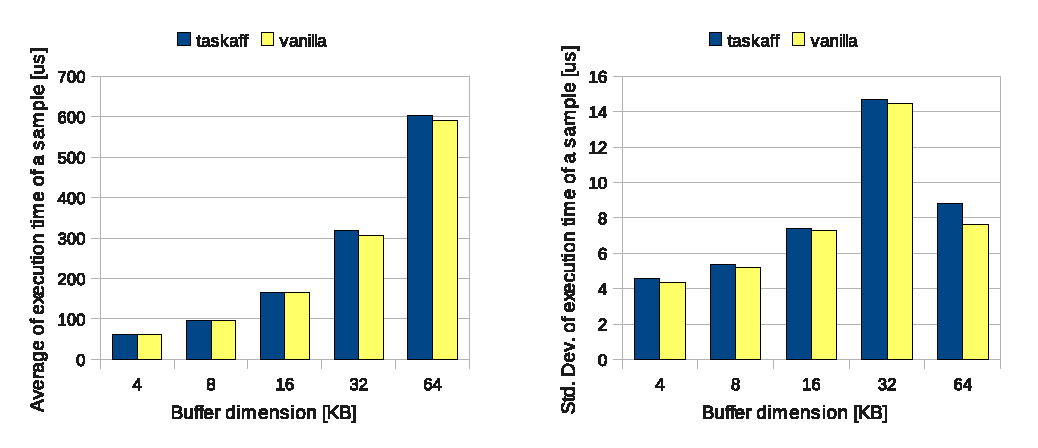
\includegraphics[width=\widefigure]{images/time/time_avg_var_Xeon.eps}
\caption{\figurecaption{Average and Variance of execution time of a sample on Xeon}}
\label{fig:avg_var_xeon}
\end{figure}

\newpage

\begin{figure}[htbp]
\centering
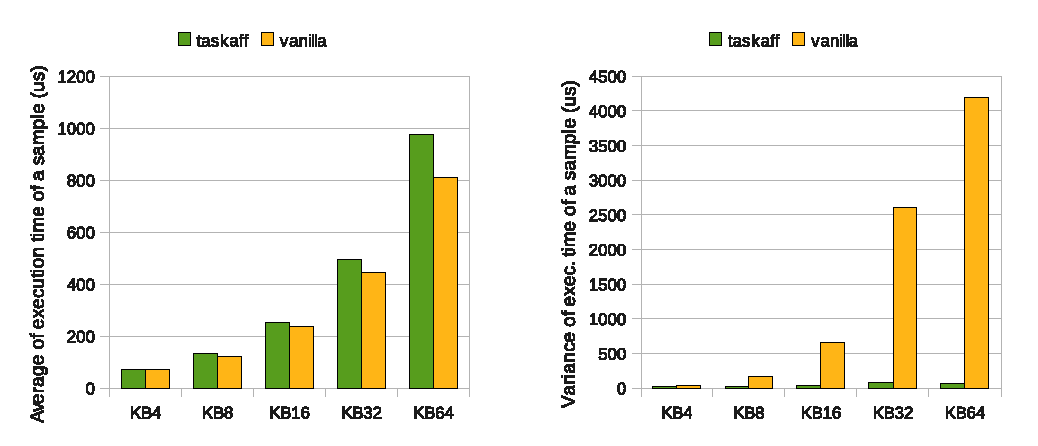
\includegraphics[width=\widefigure]{images/time/time_avg_var_i7.eps}
\caption{\figurecaption{Average and Variance of execution time of a sample on i7}}
\label{fig:avg_var_i7}
\end{figure}

\begin{table}[htbp]
\begin{center}
\begin{tabular}{l|c|c|c}
	\hline
	& Speedup \\ \hline
	& Xeon & i7 \\ \hline
	$4KB$  & -1.89\% & 2.33\% \\ \hline
	$8KB$  & -0.82\% & 6.42\% \\ \hline
	$16KB$ & -0.31\% & 8.42\% \\ \hline
	$32KB$ & -3.96\% & 6.53\% \\ \hline
	$64KB$ & -3.25\% & -5.14\% \\ \hline
\end{tabular}
\caption{Speedup obtained with task-affinity on different architectures with different buffer}
\label{tab:speedup_xeon_i7}
\end{center}
\end{table}

Speedup on Table \ref{tab:speedup_xeon_i7} is calculated in this way:

\begin{equation}
        \frac{A2S_{task\_affinity} - A2S_{vanilla}}{A2S_{vanilla}}
\label{eq:miss_rate}
\end{equation}

Where $A2S_{task\_affinity}$ and $A2S_{vanilla}$ are calculated using \ref{eq:metric_rt}.

As shown in graphics and as summarized in Table \ref{tab:speedup_xeon_i7}, the current version of task-affinity is not effective on Intel Xeon.
In terms of throughput task-affinity is not better than vanilla, because the average of execution time of a sample is about the same in both kernels 
and this is true for both the architectures. In term of predictability, on Intel i7, task-affinity is better than vanilla, especially with buffer 
greater than 32KB. Task-affinity should reduce both L1 and LLC cache misses and, consequently, improve predictability of application. But this fact 
doesn't occur on Intel Xeon. In Fig. \ref{fig:l1_load_store_Xeon} and \ref{fig:l1_load_store_i7} we can see respectively L1 read and write misses on 
Xeon and i7.

\begin{figure}[htbp]
 \centering
  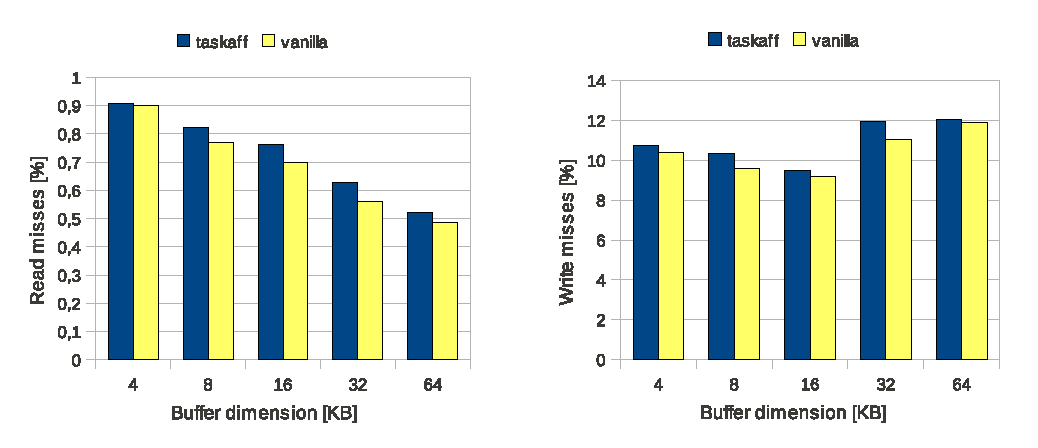
\includegraphics[width=\widefigure]{images/cache_miss/l1_load_store_Xeon.eps}
  \label{fig:l1_load_store_Xeon}
 \caption{\figurecaption{Cache miss rate of read and write instructions on Xeon}}
\end{figure}

\begin{figure}[htbp]
 \centering
  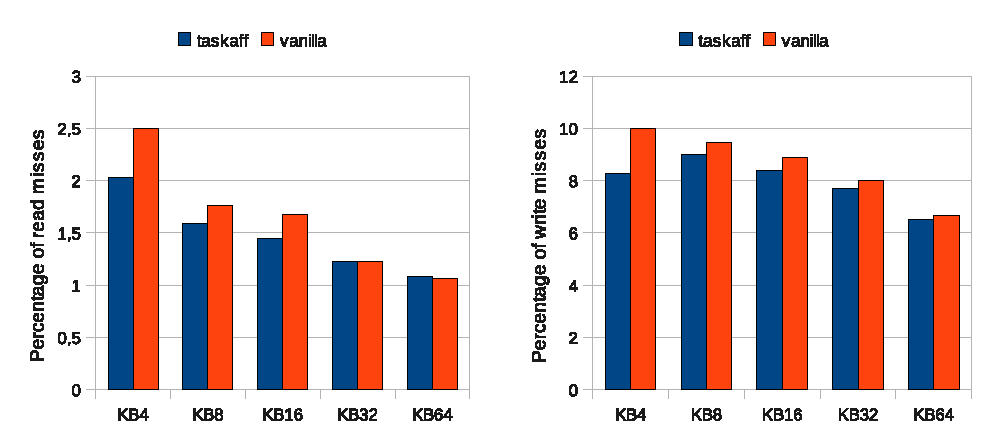
\includegraphics[width=\widefigure]{images/cache_miss/l1_load_store_i7.eps}
  \label{fig:l1_load_store_i7}
 \caption{\figurecaption{Cache miss rate of read and write instructions on i7}}
\end{figure}

On Intel Xeon read and write miss rates are increased and, consequently, predictability is degradated.

%-----------------------------------------------------------------------------
\subsection{Impact of task migration on execution time predictability}

Migration of tasks is an important factor that influences cache misses. Current version of task-affinity is not very effective in terms of reduction 
of task's migrations. As already described in \cite{lcs}, during the benchmark's execution, \textit{mixer0} or \textit{mixer1} bounce between two 
different CPUs. This issue is not related to the architecture or the buffer dimension, but it is related to the logic of task-affinity. To understand 
the reason of this problem see Fig. \ref{fig:migr_pat}.

\begin{figure}[h]
\centering
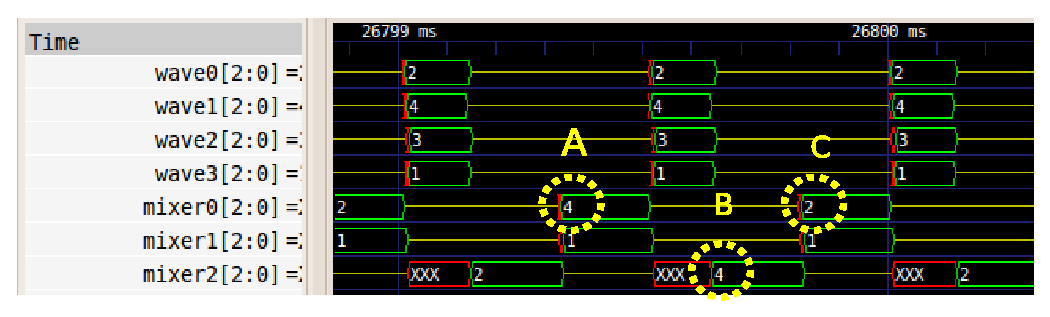
\includegraphics[width=\widefigure]{images/migr_i7.eps}
\caption{\figurecaption{Step A: mixer0 chooses cpu4. Step B: mixer2 chooses cpu4. Step C: mixer0 chooses cpu2}}
\label{fig:migr_pat}
\end{figure}

Consider step A. According to the current task-affinty logic, \textit{mixer0} has to choose a cpu that has executed \textit{wave0} or 
\textit{wave1}, that is CPU2 or CPU4, \textit{mixer2} has to choose a cpu that have executed \textit{mixer0} or \textit{mixer1}, that is CPU3 or 
CPU1. \textit{mixer0} chooses the least loaded runqeue, therefore it chooses CPU4. At Step B \textit{mixer2} can choose between CPU4 or CPU1, they 
have the same number of Real-time task, therefore \textit{mixer2} choose the first cpu in its list, that is CPU4. At step C, \textit{mixer0} has to 
choose CPU2 or CPU4 again, but it can't choose CPU4, as in step A, because it is still occupied by \textit{mixer2}, so \textit{mixer0} has to be 
executed on CPU2. This is the problem. Since \textit{mixer0} or \textit{mixer1} choose a cpu occupied by \textit{mixer2}, one of them will have to 
migrate.

Task's migration can degrade performance because a migrated task could warm up a new cache and it could create new cache interference in a new 
location already occupied by other tasks. In order to measure how much this migration pattern increases miss rate of the application, the following 
experiment was performed: two run of the benchmark are performed, in the first run all tasks are pinned on a specific cpu and they can't mirgate, in 
the second run only waves are pinned and mixers can migrate, Tab.\ref{tab:assignment} summarizes the relative cpu assignments. 

\begin{table}[tbp]
\centering%
\subfigure[All task pinned]{%
 \begin{tabular}{c|c}
	\hline
	Task & CPU \\ \hline
	Wave0 & 1  \\ \hline
	Wave1 & 2 \\ \hline
	Wave2 & 3 \\ \hline
	Wave3 & 4 \\ \hline
	Mixer0 & 1 \\ \hline
	Mixer1 & 3 \\ \hline
	Mixer2 & 3 \\ \hline
 \end{tabular} 
 \label{tab:all_pinned}
}\hspace{4em}
\subfigure[Waves pinned]{%
 \begin{tabular}{c|c}
	\hline
	Task & CPU \\ \hline
	Wave0 & 1  \\ \hline
	Wave1 & 2 \\ \hline
	Wave2 & 3 \\ \hline
	Wave3 & 4 \\ \hline
 \end{tabular} 
 \label{tab:cpuaff_waves}
}
\label{tab:assignment}
\caption{CPUs assignment}
\end{table}

What we expect with all tasks pinned and with buffer less than 32KB is a decrease of L1 read and write miss rates and a reduction of accesses to LLC. 
With dimensions greater than 32KB, the buffers can't be loaded entirely in L1 cache, therefore we don't know effect on L1 miss rates. Anyway LLC miss 
rates should diminish. With buffer less than 32KB, accesses to LLC are very different between cases with all task pinned and case with only waves 
pinned and then, miss rates that occur in two cases are not longer comparable. Note that on Intel i7, LLC is L3 and between L1 and L3 there are private L2 
caches that can store buffer of 32KB and 64KB, therefore also with buffers of 32KB and 64KB accesses to LLC should be very different in the considered cases.
But as we will see in the following graphics, also on Intel i7, in the considere cases, the number of accesses to LLC is about the same with buffer greater 
than 32KB. 

\begin{figure}[htbp]
\centering
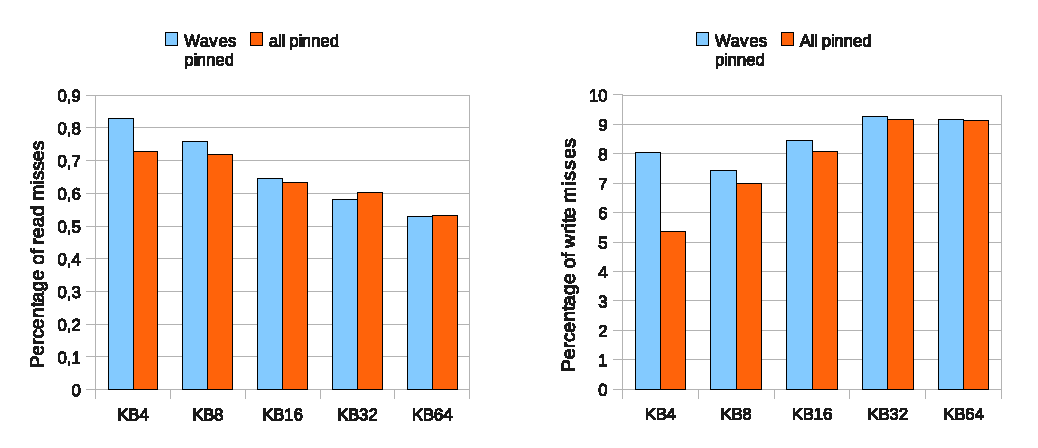
\includegraphics[width=\widefigure]{images/cpuaff/cpuaff_l1_load_store_Xeon.eps}
\caption{\figurecaption{percentage of L1 read and write misses on Xeon}}
\label{fig:cpuaff_l1_load_store_xeon}
\end{figure}

\begin{figure}[htbp]
\centering
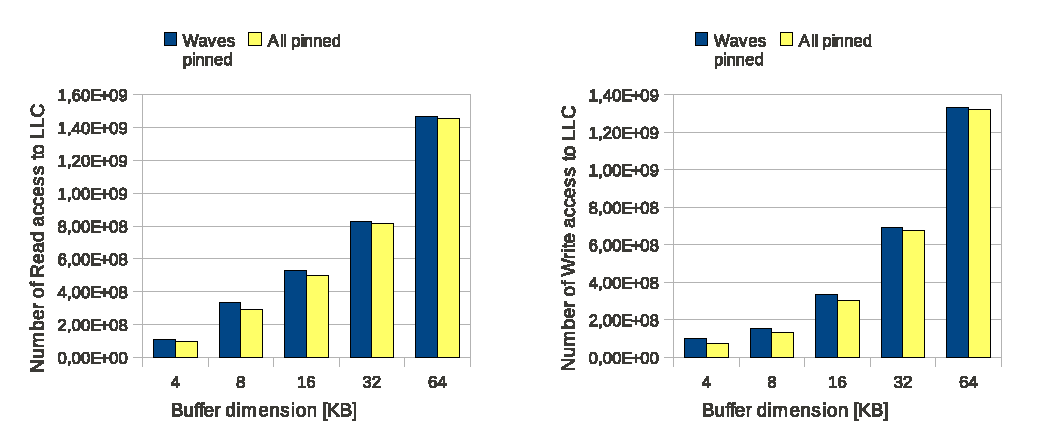
\includegraphics[width=\widefigure]{images/cpuaff/cpuaff_acc_l2_load_store_Xeon.eps}
\caption{\figurecaption{number of LLC read and write accesses on Xeon}}
\label{fig:cpuaff_acc_l2_load_store_xeon}
\end{figure}

\begin{figure}[htbp]
\centering
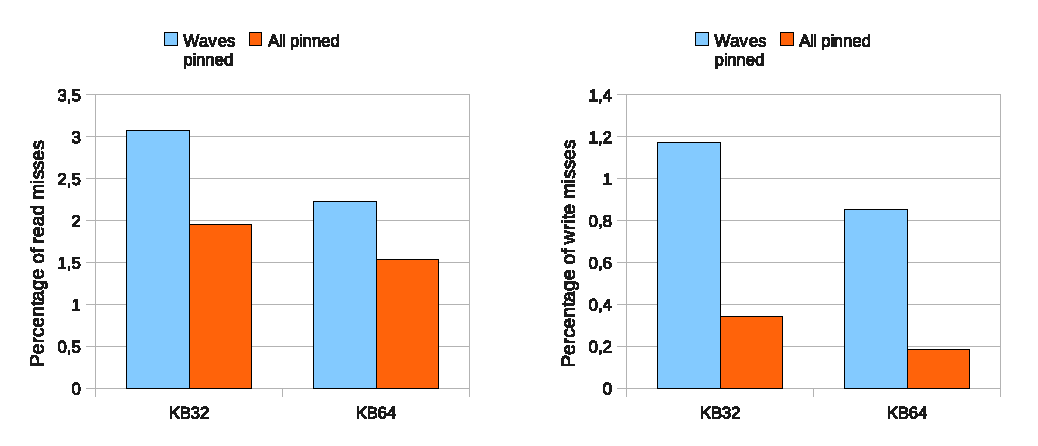
\includegraphics[width=\widefigure]{images/cpuaff/cpuaff_l2_load_store_Xeon.eps}
\caption{\figurecaption{number of LLC read and write accesses on Xeon}}
\label{fig:cpuaff_l2_load_store_xeon}
\end{figure}
\newpage

\begin{figure}[htbp]
\centering
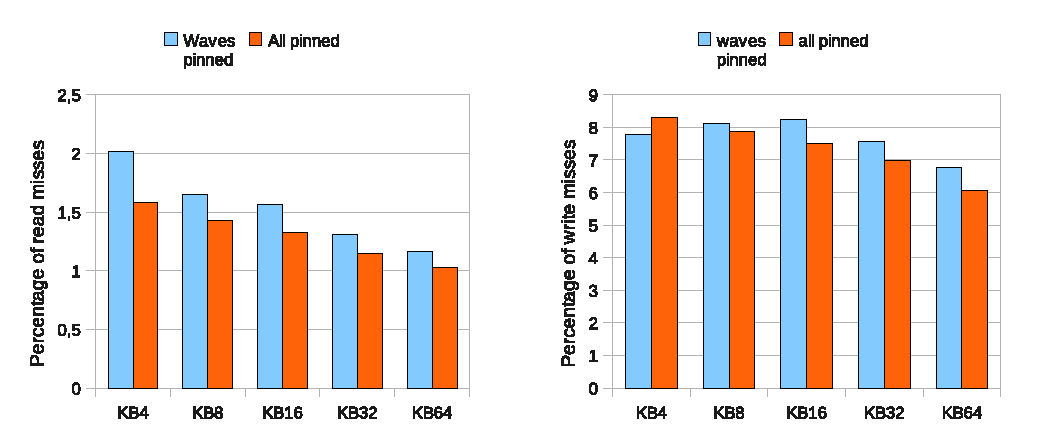
\includegraphics[width=\widefigure]{images/cpuaff/cpuaff_l1_load_store_i7.eps}
\caption{\figurecaption{percentage of L1 read miss on i7}}
\label{fig:cpuaff_l1_load_i7}
\end{figure}

\begin{figure}[htbp]
\centering
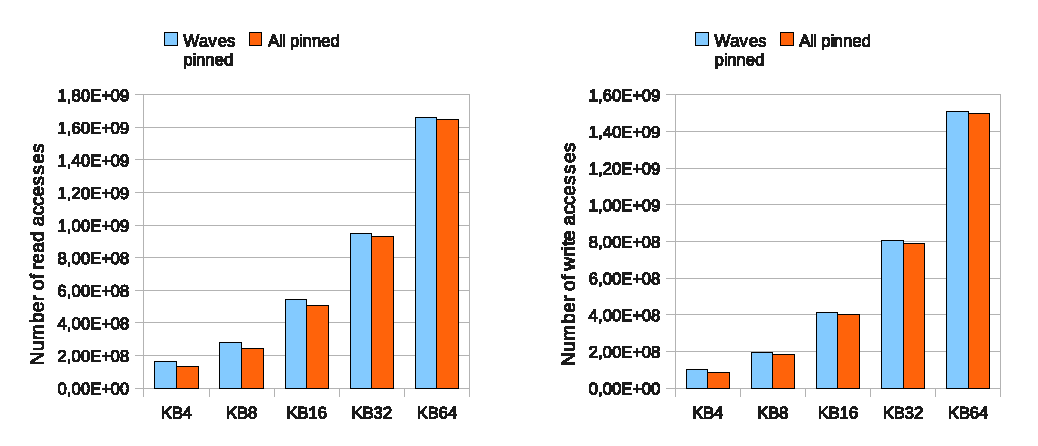
\includegraphics[width=\widefigure]{images/cpuaff/cpuaff_acc_l3_load_store_i7.eps}
\caption{\figurecaption{number of LLC read and write accesses on i7}}
\label{fig:cpuaff_acc_l2_load_store_i7}
\end{figure}

\begin{figure}[htbp]
\centering
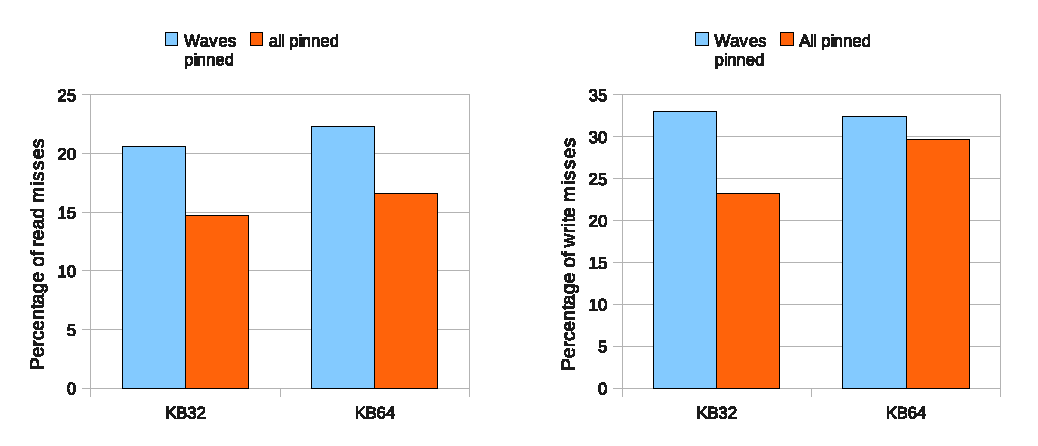
\includegraphics[width=\widefigure]{images/cpuaff/cpuaff_l3_load_store_i7.eps}
\caption{\figurecaption{percentage of LLC read miss on i7}}
\label{fig:cpuaff_l1_load_i7}
\end{figure}

\newpage
%-----------------------------------------------------------------------
\subsection{Considerations on experimental results}

We can infer from these graphics, that migration pattern have a great influence on read/write miss rate on LLC in both architectures considered. 

On Intel Xeon, L1 and LLC read and in particular write misses are greatly increased, this fact is due to cache architecture. On Xeon cores are not all on 
the same die, for example: assume that core 1 and 2 are on the same die, while core 3 and 4 are on the other die. If a task is executed on core 1 and 
request a data on core 3, that request will result in a miss, therefore if a task bounces from CPUs that own to different dies, each time it has to warm 
up the cache. This issue regards especially write operations, because for read operations, hardware prefetchers mitigate this problem.

On Intel i7, instead all core share a common LLC. When a core requires a data, it sends a data request to L3 cache. If data is in L3 and there is a hit, 
the L3 cache query the "core valid" bits of the cache line that contains requested data, in order to know which is the core that owns requested data. The 
core that owns requested data reply to the request with the most recent copy of data. For this reason, each core on i7 can use data in other private cache
because all data are contained in LLC.

To get a sense on how much cache miss influence predictability of the application, see Fig. \ref{fig:time_cpf_var_Xeon_i7}. In the graphics two run of the
benchmark are compared: in the first run all tasks are pinned, while in the second run all tasks can migrate according migration policy of vanilla kernel.

\begin{figure}[htbp]
\centering
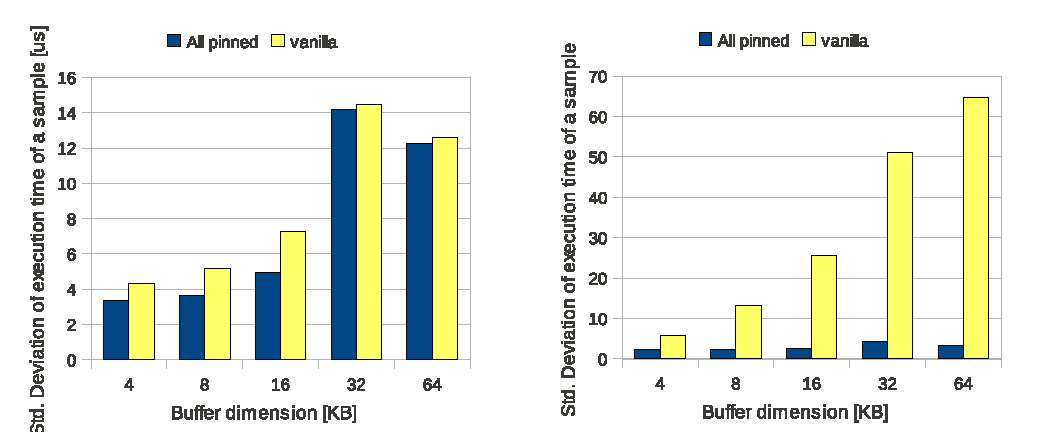
\includegraphics[width=\widefigure]{images/cpf_time/time_cpf_var_Xeon_i7.eps}
\caption{\figurecaption{variance of execution time of a sample on Xeon and i7: all task pinned compared vanilla}}
\label{fig:time_cpf_var_Xeon_i7}
\end{figure}

It is interesting to note how the absence of migration improve the predictability when buffer used are greater than 32KB that can't be stored in L1 but 
only in LLC cache or in private L2 (Intel i7).

Performance degradation on Intel Xeon is not only due to migration pattern. As I said before, cache architectures of Xeon and i7 are very different and
from previous graphics seems that with cache architecture of Intel i7, task-affinity is more effective, but there is another important aspect that 
influences performace: it is \textbf{Inter-chip communication}. Intel i7 use the new Quick-path Interconnect that is a point-to-point processor 
interconnect developed by Intel to compete with HyperTransport. This first implementation of this bus achieve 25.6 GB/s, which provides exactly double the 
theoretical bandwidth of Intel's 1600 MHz FSB, that is the best performance obtainable with FSB. From datasheet, Intel Xeon E5440 use a FSB at 1333 MHz, 
therefore communication between chips are more faster on i7. Hence, it is clear that communication between cores that belong to different dies is very 
expensive on Intel Xeon. On Intel Xeon, \textit{mixer0} or \textit{mixer1} could find one buffer in L1 cache and other buffer in a bank of L2 that is 
shared by the cpu that have execute it. \textit{Mixer2} could find one buffer on L1 one cache, while other buffer is \textit{always} placed on bank of L2 
that is not shared by the cpu that has executed \textit{Mixer2}, therefore read latencies are very high, because data are placed on different dies. 
On i7, instead, \textit{mixer2} could find one buffer in L1 cache and other buffer in L3 cache that is shared among all cores and it is inclusive, 
therefore to read data is less expensive on i7.

%%%%%%%%%%%%%%%%%%%%%%%%%%%%%%%%%%%%%%%%%%%%%%%%%%%%%%%%%%%%%%%%%%%%%%%%%%%%%
\section{Task-affinity improvements}

Before to explain how the new kernel patch works, it is necessary to remember the concept of task-affinity. We say that two tasks have a task-affinity 
relationship if they share data and their execution depends upon reading or writing this data \cite{lcs}. In a producer-consumer application, the 
producer is the one that writes to the shared buffer, while the consumer is the one that reads it. The consumer depends on data generated by the producer 
since it needs it in order to be able to run, therefore we say that the consumer has a task-affinity relationship toward the producer.

\begin{figure}[htbp]
\centering
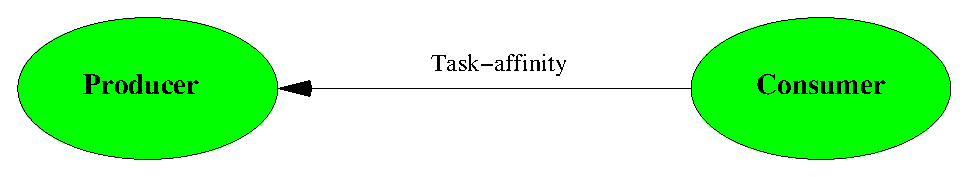
\includegraphics[width=\widefigure]{images/taskaff-rel.eps}
\caption{\figurecaption{Task-affinity relationship between producer and consumer}}
\label{fig:taskaff-rel}
\end{figure}

Each task is provided with a linked list called \textit{taskaffinity\_list} that contains all tasks to which it has task-affinity relationship, briefly 
all its producers. To insert and delete a task in a \textit{taskaffinity\_list} two new system calls are provided:

\begin{description}

\item[sched\_add\_taskaffinity:] This system call adds a dependency to the current task, i.e. the task that issued the call. It receives, as parameter, the 
pid of the task the current one will be dependent upon.

\item[sched\_del\_taskaffinity:] When a task does not want anymore to use the task-affinity mechanism, it is possible to remove it through this call.
As in the case of inclusion of dependency, it suffices to pass as parameter the pid of the task one wants not to follow anymore.

\end{description}

Thanks to these system calls, the scheduler "knows" which tasks have task-affinity and, in this way, it can schedule consumers after producers in order to 
enforce reuse of cache memory.

The task-affinity logic influences wake up and migration of a task. As we have previously seen, in \textit{try\_to\_wake\_up} the choice of cpu where to 
put the to be waken task is made by \texttt{select\_task\_rq\_rt} \ref{code:select_task}. This function is modified in this way: given the input task $p$, 
the function doesn't call \texttt{find\_lowest\_rq} but it loops for all element present in the $p$'s \textit{taskaffinity list} and build a mask, called 
\textit{affinity\_mask}, with cpus that have executed a task present in $p$'s \textit{taskaffinity\_list}. Finished the loop, the function returns the cpu 
with the runqueue that has the lowest number of Real-Time tasks. Only if the mask is empty, the function calls \texttt{find\_lowest\_rq} to choose a cpu
in the standard way. 

In the current version of task-affinity, a task that "respect" task-affinity, that is a task that was enqueued according to its task-affinity 
relationships, isn't able to migrate. In plain words, \texttt{push\_rt\_task} and \texttt{pull\_rt\_task} can't move tasks that "respect" task-affinity.

The aim of this policy is clear: when a task wakes up, the policy tries to select the best cpu for that task and, if it finds it, it blocks the task on the 
best runqueue until the task's execution. For this reason the key point of this task-affinity logic is the \texttt{select\_task\_rq\_rt}. In the optimal 
case, producers and consumers will be executed subsequenlty always on the same cpu.

Nevertheless, in practice, the choosen cpu for $p$ is next to never the optimal cpu. The reason is very simple. The choice of the best 
cpu, and the enqueuing of task are performed in different moments. When \texttt{select\_task\_rq\_rt} is called, it doesn't hold any lock. During the loop, 
the function has to read what is the content of different runqueues present in the system, these reads are not synchronized. Once the cpu is selected, 
\texttt{select\_task\_rq\_rt} returns and \texttt{try\_to\_wake\_up} \textbf{takes a lock} on the choosen runqueue, in order to call 
\texttt{activate\_task} to perform the enqueuing of the task. From when \texttt{select\_task\_rq\_rt} selects the cpu to when the lock is taken, a task 
with equal or higher priority than $p$'s priority can be inserted in the selected runqueue and, in this way, the next task that will be executed won't be 
$p$. 

The current version of task-affinity ensures only weak concept of temporal locality because it doesn't ensure, when it is possible, that the next task 
executed after a producer is a consumer. Another problem of the current version of task-affinity is the migration policy. It is not very flexible. Pull 
and push functions mantain the system balanced, and guarantee that every cpu executes always the higher priority Real-time task present in its runqueue.
Therefore, the denial to pull and push can improve predictability of the application and can degrade singnificantly the throughput of the application.
Predictability is an important aspect for Real-time systems, but if we have a very bad throughput we don't exploit the potentiality of multicore platforms.

The aim of the patch developed in this thesis is to improve the concept of temporal locality in order to execute a consumer immediately after a 
producer, when it is possible and to improve the migration policy in order to use also the functions involved in the migration mechanism to exploit the 
concept of task-affinity. Furthermore, the patch makes task-affinity more robust synchronizing the accesses to data structures used. With this patch we 
try to improve throughput and predictability of the application. 

%%%%%%%%%%%%%%%%%%%%%%%%%%%%%%%%%%%%%%%%%%%%%%%%%%%%%%%%%%%%%%%%%%%%%%%%%%%%%
\section{Patch structure}

The proposed patch is divided in two parts. The first part improves the temporal locality, while the second part introduces mechanisms to synchronize 
accesses to task-affinity data structures.

%-----------------------------------------------------------------------------
\subsection{Temporal locality}

The implemented logic to improve temporal locality is divided in the following parts:

\begin{description}

\item[last\_tsk field] To ensure that a consumer will be the next executed task after a producer, it is necessary to change what 
\texttt{select\_task\_rq\_rt} "sees". As I previously said, during its loop, \texttt{select\_task\_rq\_rt} checks for CPUs that \textbf{have executed} a 
task in $p$'s \textit{taskaffinity list}. It means that, in that moment, those cpus could be executing a task that is not a producer and such, the L1 cache 
could already be dirty. For this reason, at each runqueue was added a field named \texttt{last\_tsk} that contains the last task executed in a runqueue. 
This field is updated at each context switch if the next task to be executed is different from idle. In this way, if current task on runqueue is not idle, 
this field represents, the task in execution. With this additional field, \texttt{select\_task\_rq\_rt} "knows" which is the task currently executing on 
each runqueue. In this way, cpus that during \texttt{select\_task\_rq\_rt} are executing a task that is not in $p$'s \textit{taskaffinity\_list} are not 
inserted in \texttt{affinity\_mask}.

\item[enqueue on head] This change is not enough. Consider this situation: two different cpus that we call CPU\_A and CPU\_B are executing two different 
istances of \texttt{try\_to\_wake\_up}. Respectively, they are called for task $p$ and task $q$: the former has task-affinity relationship, the latter is 
a generic Real-time task, both tasks have the same priority. Suppose that the current task on CPU\_A is a task in $p$'s \textit{taskaffinity list} and then 
\texttt{select\_task\_rq\_rt} choose CPU\_A for $p$. Suppose that \texttt{try\_to\_wake\_up} that wakes up $q$ chooses CPU\_A and enqueue task $q$ on the 
runqueue of CPU\_A. Task $p$ is not yet enqueued, therefore when it will be enqueued, it will be preceeded by $q$ and then the next task that will
be executed on CPU\_A is $q$.

\begin{figure}[htbp]
\centering
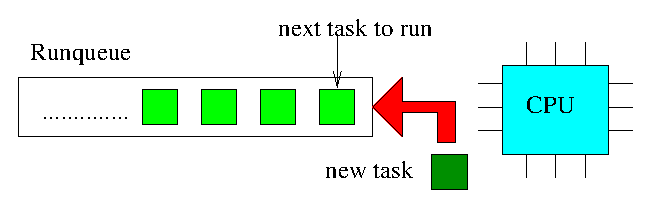
\includegraphics[width=10cm,height=12cm, keepaspectratio]{images/enq_head.eps}
%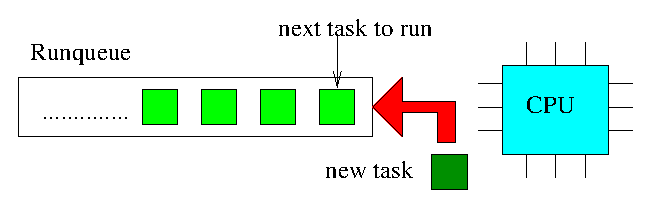
\includegraphics[width=\widefigure]{images/enq_head.eps}
\caption{\figurecaption{Enqueue on head}}
\label{fig:enq_head}
\end{figure}

To resolve this problem a task that "respects" task-affinity is enqueued on the top of a runqueue and not on its tail. In this way, if two Real-time tasks 
are on the same runqueue and have the same priority, but one of them "respects" a task-affinity, the next task that will be executed is the task that 
"respects" a task-affinity. 

\item[choice of current task] Even if a task with task-affinity is enqueued on head in a runqueue, it will be the next executed task only if it is 
enqueued before it is executed a task that is already on that runqueue. For this reason, it is necessary to optimize the choice made in 
\textit{select\_task\_rq\_rt}. In \texttt{select\_task\_rq\_rt}, when a task with task-affinity, that we call $p$, has built its \textit{affinity mask}, 
it checks if in that mask there is the CPU that is executing the \texttt{try\_to\_wake\_up} that are waking up it. If this is true, it means that the 
current task on that CPU is a $p$'s producer and now on that CPU a \texttt{try\_to\_wake\_up} is in execution, therefore any other task enqueued on that 
CPU in that moment can't be executed, because during \texttt{try\_to\_wake\_up} kernel preemption is disabled and then it is necessary wait that 
\texttt{try\_to\_wake\_up} finish. Choosing that CPU, $p$ will be the next task executed on that CPU, because it is enqueued on head and it can precede 
all task enqueued on that CPU during \textit{select\_task\_rq\_rt}.

\item[migration mechanism] There is another a problem. It could happen that a task with higher priority is enqueued on the same runqueue where a task with 
task-affinity is enqueued. In this case, the next task to execute won't be the task with task-affinity.
To resolve this problem, migration mechanism is used. When the \texttt{try\_to\_wake\_up} has enqueued task $p$ it calls function \texttt{task\_woken} in 
order to checks if $p$ can be immediately executed on the selected runqueue or not. If on the runqueue there is a task with priority equal or higher than 
the $p$'s priority and this task precedes $p$, \texttt{push\_rt\_task} is called and $p$ can be pushed on another cpu. To select the cpu where to push $p$, 
the same mechanism used in \texttt{select\_task\_rq\_rt} is adopted. Therefore, $p$ will be pushed where it is in execution a task in $p$'s 
\textit{taskaffinity\_list}, if it is impossible standard push criteria are adopted and $p$ will be pushed on a cpu that executing a task with lower 
priority than $p$. Obviously, in order to push a task that "respect" task-affinity, it is necessary insert it in a \textit{pushable list}. 

\end{description}
%-----------------------------------------------------------------------------
\subsection{Synchronization}

In the current version of task-affinity, accesses to data structures used to manage task-affinity are made by user or by kernel. The resource that must be
synchronized is \texttt{taskaffinity\_list}

\begin{description}

\item[Access from user space:] User can access to task-affinity data structures using syscalls \texttt{sched\_add\_taskaffinity}, and 
\texttt{sched\_del\_taskaffinity}. These functions access the pid of the task received in input in synchronized way, by using the read-write lock
tasklist\_lock that protects the kernel's internal task list. For this reason, at every moment, only one instance of these syscalls can modify the
task-affinity data structure of a task.

\item[Access from kernel space:] Here the situation is more complex. There are two functions that can access to task-affinity data structures, they are:
\texttt{task\_affinity\_notify\_exit} and \texttt{select\_task\_rq\_rt}. The former function frees task-affinity data structures and is called when a 
task is exiting. During this phase, all resources used by a task, pid included, are deallocated. Therefore, when \texttt{task\_affinity\_notify\_exit} is 
called, \textit{tasklist\_lock} is acquired. This is not enough because in that moment \texttt{select\_task\_rq\_rt} could access the task-affinity data 
structures of the exiting task, for this reason another layer of synchronization is needed. To resolve this problem, each task has its own read-write lock 
named \textit{taskaff\_lock} to protect its task-affinity data structures. 

\end{description}

